\documentclass[12pt]{ctexart}
\usepackage{amsmath, amssymb, enumitem, xcolor, graphicx, multicol, float}

\begin{document}

\section*{试卷一}
\begin{enumerate}[label=\arabic*.]
    \item 计算:$\left|\sqrt{6}-\sqrt{3}\right|+\left|2-\sqrt{6}\right|=$
    \item 已知$a,b$互为相反数,$c,d$互为倒数,$m$的倒数等于它本身,求$\dfrac{cd}{m^2}+(a+b)m-m$的立方根.
    \item 在$\sqrt{2},-(-2),\sqrt[3]{-8},-|- \sqrt{2}|$中,最小的数是()
    \item 比较大小:$3\sqrt{27}$ $\_\_\_\_$ $\sqrt{162}$.
    \item 解方程:$(x-1)^2-49=0$;
    \item 已知一个数的平方根是$3a+1$和$a+11$,则这个数的立方根是 $\_\_\_\_$ .
    \item 如果$\sqrt{16}$的算术平方根是$-m$,$-64$的立方根是$n$,那么$m-n=$ $\_\_\_\_$ .
    \item 如果$x^2=1$,那么$\sqrt[3]{x}$的值是 $\_\_\_\_$ .
    \item 计算$|1-\sqrt{2}|$的结果是()
    \item 已知$a,b,c$为实数,且它们在数轴上的对应点的位置如图所示,化简$2\sqrt{(b-a)^2}+|b+c|-\sqrt{(a-c)^2}-2|a|$.
    \item 把无理数$\sqrt{11},\sqrt{5},-\sqrt{3}$表示在数轴上,在这三个无理数中,被墨迹(如图所示)覆盖住的无理数是 $\_\_\_\_$ .
    \item M,N两点同时出发相向而行,在原点处相遇,求N点的运动速度;
    \item M,N两点按上面的各自速度同时出发,向数轴正方向运动,几秒时两点相距6个单位长度;
    \item M,N两点按上面的各自速度同时出发,向数轴负方向运动,与此同时,C点从原点出发沿同方向运动,且在运动过程中,始终有$CN:CM=1:2$.若干秒后,C点在$-12$处,求此时N点在数轴上的位置.
    \item 阅读材料并解决下列问题:
        \begin{enumerate}
            \item $[\sqrt{2}]=$ $\_\_\_\_$ ;
            \item 若$[3+\sqrt{x}]=6$,则$x$的取值范围是 $\_\_\_\_$ .
        \end{enumerate}
\end{enumerate}

\begin{figure}[H]
    \centering
    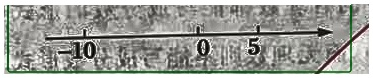
\includegraphics[scale=0.5]{cropped_1.jpg}
    \caption{数轴示意图}
\end{figure}

\newpage

\section*{试卷二}
\begin{enumerate}[label=\arabic*.]
    \item 解方程:$(x-1)^2-49=0$;
    \item 已知一个数的平方根是$3a+1$和$a+11$,则这个数的立方根是 $\_\_\_\_$ .
    \item 如果$\sqrt{16}$的算术平方根是$-m$,$-64$的立方根是$n$,那么$m-n=$ $\_\_\_\_$ .
    \item 如果$x^2=1$,那么$\sqrt[3]{x}$的值是 $\_\_\_\_$ .
    \item 计算$|1-\sqrt{2}|$的结果是()
    \item 已知$a,b,c$为实数,且它们在数轴上的对应点的位置如图所示,化简$2\sqrt{(b-a)^2}+|b+c|-\sqrt{(a-c)^2}-2|a|$.
    \item 把无理数$\sqrt{11},\sqrt{5},-\sqrt{3}$表示在数轴上,在这三个无理数中,被墨迹(如图所示)覆盖住的无理数是 $\_\_\_\_$ .
    \item M,N两点同时出发相向而行,在原点处相遇,求N点的运动速度;
    \item M,N两点按上面的各自速度同时出发,向数轴正方向运动,几秒时两点相距6个单位长度;
    \item M,N两点按上面的各自速度同时出发,向数轴负方向运动,与此同时,C点从原点出发沿同方向运动,且在运动过程中,始终有$CN:CM=1:2$.若干秒后,C点在$-12$处,求此时N点在数轴上的位置.
    \item 阅读材料并解决下列问题:
        \begin{enumerate}
            \item $[\sqrt{2}]=$ $\_\_\_\_$ ;
            \item 若$[3+\sqrt{x}]=6$,则$x$的取值范围是 $\_\_\_\_$ .
        \end{enumerate}
\end{enumerate}

\begin{figure}[H]
    \centering
    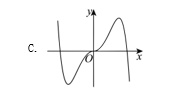
\includegraphics[scale=0.5]{cropped_2.jpg}
    \caption{数轴示意图}
\end{figure}

\newpage

\section*{试卷三}
\begin{enumerate}[label=\arabic*.]
    \item 解方程:$(x-1)^2-49=0$;
    \item 已知一个数的平方根是$3a+1$和$a+11$,则这个数的立方根是 $\_\_\_\_$ .
    \item 如果$\sqrt{16}$的算术平方根是$-m$,$-64$的立方根是$n$,那么$m-n=$ $\_\_\_\_$ .
    \item 如果$x^2=1$,那么$\sqrt[3]{x}$的值是 $\_\_\_\_$ .
    \item 计算$|1-\sqrt{2}|$的结果是()
    \item 已知$a,b,c$为实数,且它们在数轴上的对应点的位置如图所示,化简$2\sqrt{(b-a)^2}+|b+c|-\sqrt{(a-c)^2}-2|a|$.
    \item 把无理数$\sqrt{11},\sqrt{5},-\sqrt{3}$表示在数轴上,在这三个无理数中,被墨迹(如图所示)覆盖住的无理数是 $\_\_\_\_$ .
    \item M,N两点同时出发相向而行,在原点处相遇,求N点的运动速度;
    \item M,N两点按上面的各自速度同时出发,向数轴正方向运动,几秒时两点相距6个单位长度;
    \item M,N两点按上面的各自速度同时出发,向数轴负方向运动,与此同时,C点从原点出发沿同方向运动,且在运动过程中,始终有$CN:CM=1:2$.若干秒后,C点在$-12$处,求此时N点在数轴上的位置.
    \item 阅读材料并解决下列问题:
        \begin{enumerate}
            \item $[\sqrt{2}]=$ $\_\_\_\_$ ;
            \item 若$[3+\sqrt{x}]=6$,则$x$的取值范围是 $\_\_\_\_$ .
        \end{enumerate}
\end{enumerate}

\begin{figure}[H]
    \centering
    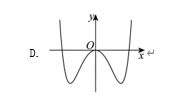
\includegraphics[scale=0.5]{cropped_3.jpg}
    \caption{数轴示意图}
\end{figure}

\end{document}